\lhead{\emph{State of the Art}}
\section{State-of-the-art of Error Correction Code}
\subsection{Related works}
\subsection{ECC for Optical Interconnects}

Instead of deploying a WSN to monitor all devices in home as in ILM, a hybrid system uses less sensors to detect the environmental parameters and infer the state of some specific devices, while the others are still identified by an NILM algorithm. 
In order to reduce the computational complexity while still ensuring the accuracy for load monitoring, in \cite{TangW16}, the occupancy is considered as a significant external feature because a part of devices operates during occupied periods. Figure~\ref{fig:A13} illustrates the correlation between the operation of some devices and the occupancy in home. Therefore, the NILM algorithms can be applied only when the occupancy monitoring system, as introduced in Chapter \ref{Introduction}, detects an occupancy. By cutting out the unoccupied periods, the computational complexity can significantly decrease, particularly if the unoccupied periods are dominating. Obviously, the detection accuracy also decreases if there are too many background loads or automatically fluctuated devices such as fridge, washing machine, dish washer, heater, etc. Meanwhile, in \cite{Berges10,Berges11,Guvensan13}, the environmental parameters such as light intensity or audio signal are analyzed to give conclusion on the operation of some specific devices, e.g. the variations in acoustic signal relate to the operation of an air blower and a refrigerator as shown in Figure~\ref{fig:AA13}. Instead of installing new sensors, the embedded sensors of mobile phones can also be used to fingerprint the profile of each device~\cite{Uddin12}. Although the hybrid approach allows to increase the performance of load monitoring systems, more algorithms must be studied for sensors signal processing.

\begin{figure}[!ht]
\centering
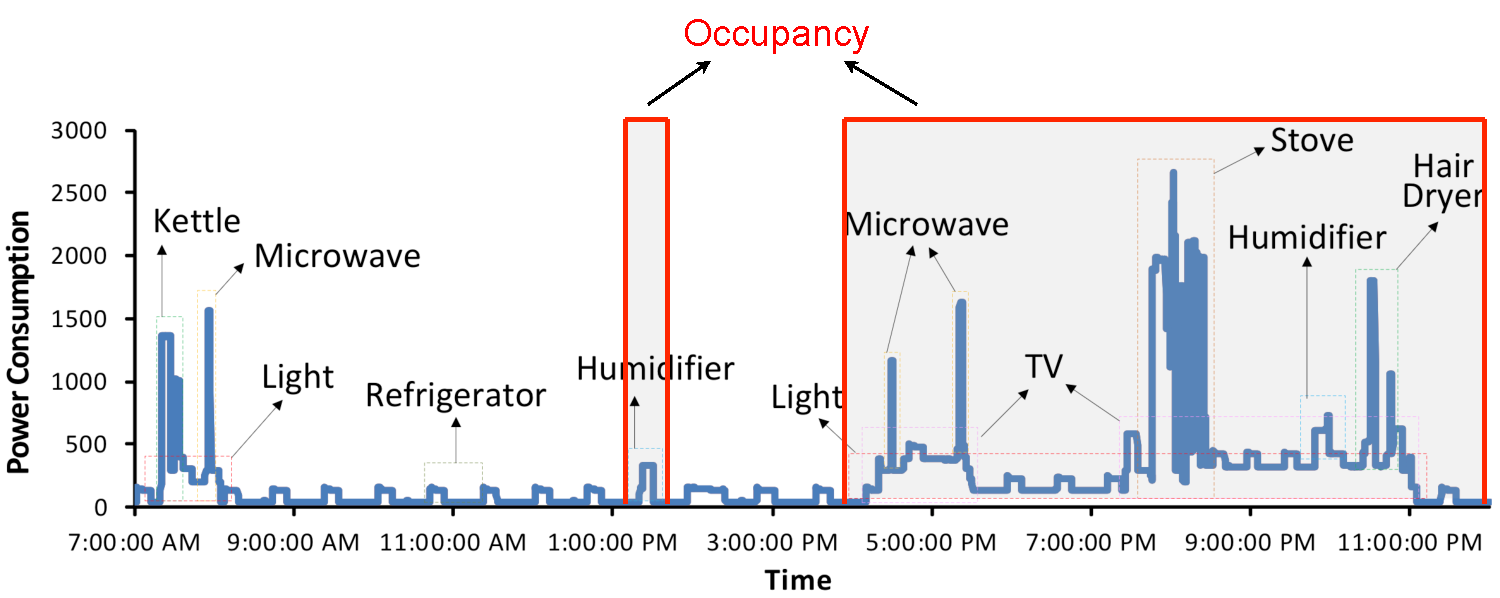
\includegraphics[width=1\textwidth]{./chapters/chapter2/images/occupancy_states.pdf} 
\caption{Power consumption with and without the occupants~\cite{TangW16}.} 
\label{fig:A13} 
\end{figure}

\begin{figure}[!ht]
\centering
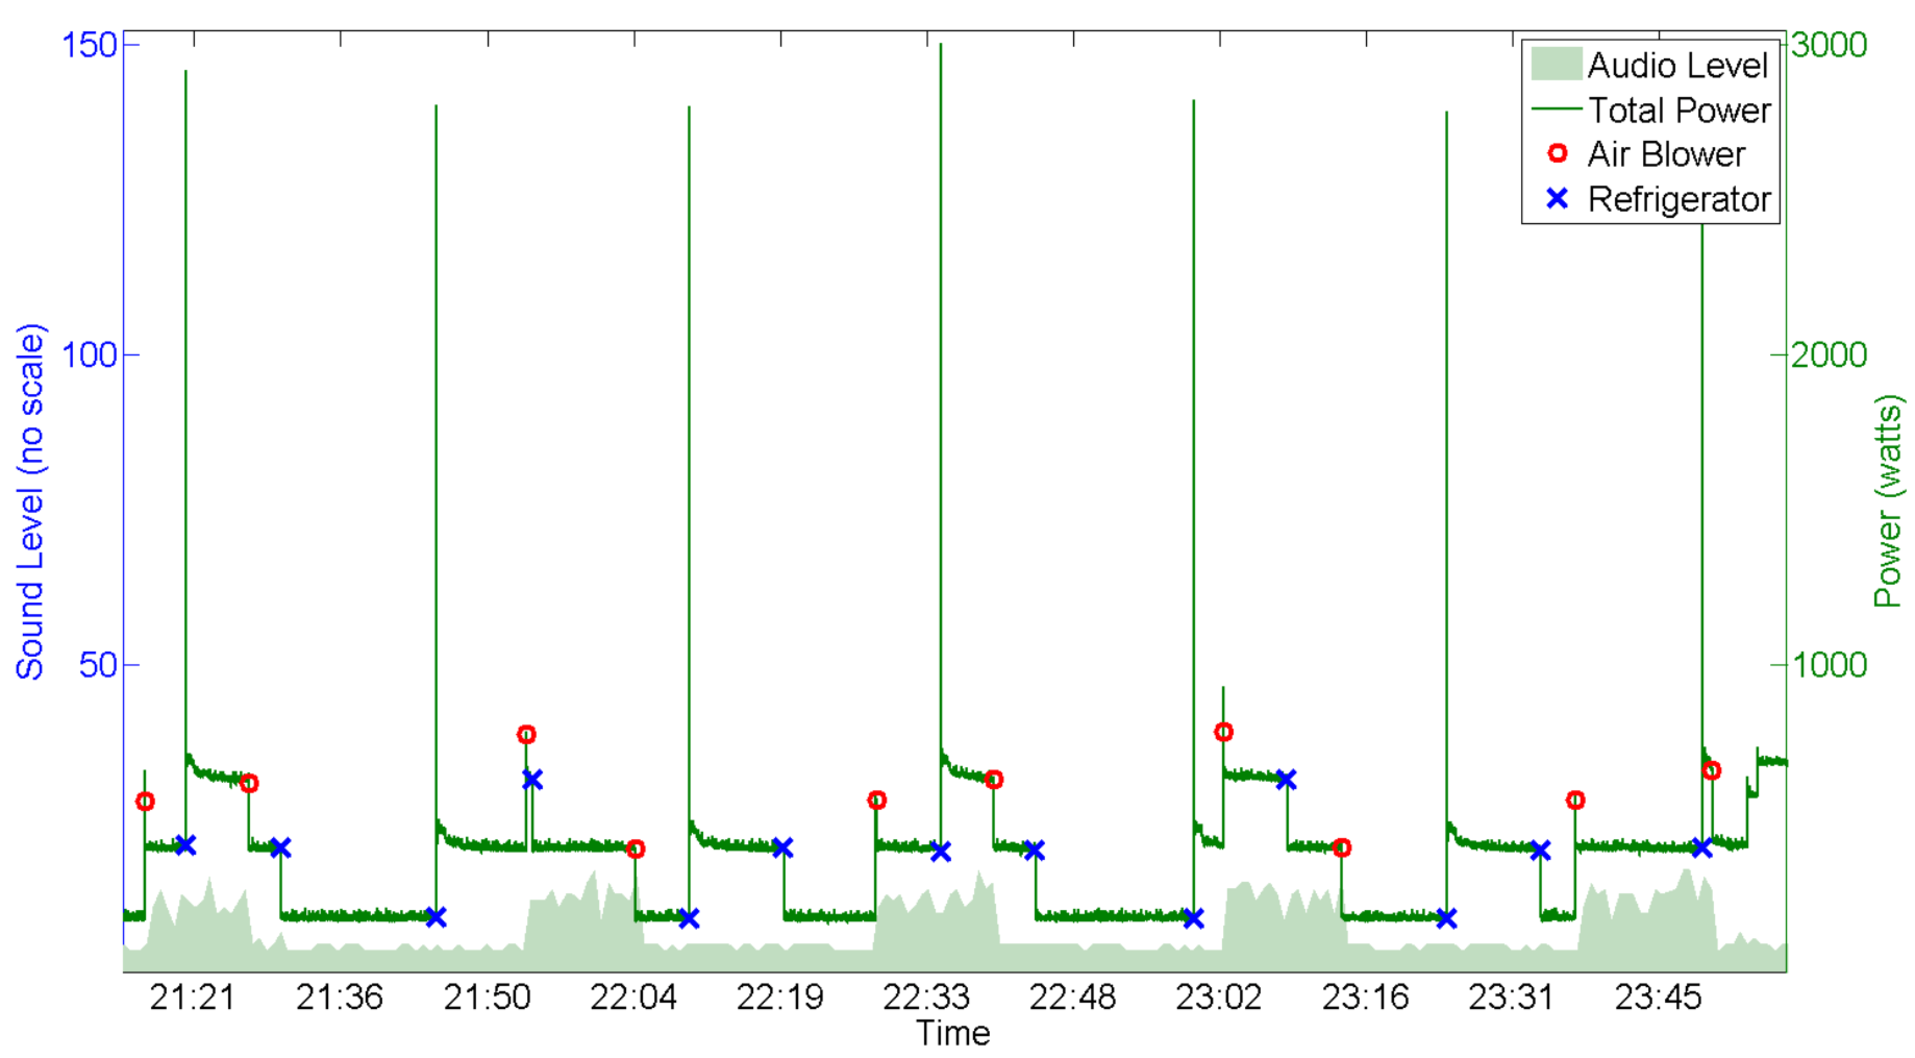
\includegraphics[width=1\textwidth]{./chapters/chapter2/images/audiochange.pdf} 
\caption{Aggregate power consumption and the variation of audio signal in a living room~\cite{Berges10}.} 
\label{fig:AA13} 
\end{figure}



\section{Conclusions}
In this chapter, we have an overview on the load monitoring including intrusive, non-intrusive and hybrid approaches. ILM is the most accurate approach, but it needs very large amount of sensors to monitor all electrical consumers and therefore it is impossible to be widely applied. Meanwhile, non-intrusive approaches help to significantly reduce the deployment cost as well as technical intervention on the power supply. Nevertheless, ambiguity in the power characteristics of the devices is the most important problem in an NILM system and prevents the system from increasing the performance. As a consequence, HLM can be considered as a compromise between two approaches, which can reduce the deployment cost of ILM and increase the performance of NILM. In this thesis, we will study on hybrid methods, which use external information such as state transition probability or operating probability of each device to improve the performance of existing NILM algorithms. Concretely, in Chapter 3, we propose to use the state transition of each device from previous instant to current instant as an external information and combine it to the minimization problem in Eq.~\eqref{eqI7}. Meanwhile, in Chapter 4, we introduce SmartSense model, in which a WSN is deployed to monitor the operation of a subset of all devices. Sensor detection is then transformed to the operating probability of corresponding devices. Disaggregation algorithms use this probability along with other specific features extracted from the global power signal to determine the state of each device.























